\clearpage
\chapter{\textbf{Grundlagen}}\label{grundlagen}
%\addtocontents{toc}{\vspace{0.8cm}}

\section{Machine Learning}\label{unterkapitel}
\addtocontents{toc}{\vspace{0.8cm}}

Grundsätzlich beschreibt Machine Learning das Entwickeln mathematischer Modelle zur statistischen Auswertung
von Daten. Dabei wird dem Modell anhand von Daten zu einem bestimmten Sachverhalt beigebracht, in einem 
Datenset Schemata zu erkennen, womit sich eine Erwartung über die Umstände des Datensets treffen lässt.
Beispielsweise könnte ein solches Model aus einem Datenset mit der aktuellen Jahreszeit, Uhrzeit und 
Position der Sonne am Himmel trainiert werden, sodass es auch schließlich in einem anderen Datenset 
aus Jahreszeit und Position der Sonne Rückschlüsse auf die Uhrzeit treffen kann.\\
Als Vorbild für diesen ,,Lernvorgang'' dient das menschliche Gehirn, welches ebenfalls versucht zwischen 
bestimmten Input-Parametern wie z.B. der Form und Farbe eines Gegenstandes eine Beziehung herzustellen,
um das beobachtete Objekt in Zukunft schneller kategorisieren zu können.\\
Da eine Vielzahl von effektiven Machine Learning Algorithmen existiert, ist es essenziell, sich mit den
Stärken und Schwächen einzelner Herangehensweisen zu befassen.\newpage

Im Wesentlichen kann Machine Learning in zwei Unterkategorien unterteilt werden:
\begin{itemize}
    \item \textit{Supervised Learning} 
    \item \textit{Unsupervised Learning}
\end{itemize}
\textit{Supervised Learning} bedeutet zwischen bestimmten Feldern eines Datensets eine Beziehung
zu einem sog. Label herzustellen, welches als eine Art Ergebnis aus den Eingabewerten gesehen 
werden kann. Ein so traniertes Model kann dann neue, ihm vorher unbekannte Datensets, mit einem 
Label versehen - etwa wie in dem o.g. Beispiel wo Jahreszeit und Sonnenposition die Eingabewerte 
und die Uhrzeit das Label darstellen. Der Begriff ,,\textit{supervised}'' ergibt sich daraus, dass 
das Datenset, mit dem das Model traniert wird, diese Labels gegeben 
hat, sodass das Modell sich bei jedem Schritt des Lernvorgangs selbst korrigieren kann, falls 
eine Fehleinschätzung getroffen wurde.
Bei einer sog. ,,\textit{Klassifizierung}'' sind diese Labels fest vorgegeben, während sie in der 
,,\textit{Regression}'' kontinuierlicher Natur sind. Im Kontext dieser Arbeit wäre das Ergebnis einer 
Klassifizierung eine ,,1'' für Anwesenheit und eine ,,0'' für Abwesenheit, während das Ergebnis einer 
Regression eine Wahrscheinlichkeit auf Anwesenheit zwischen 0.0 und 1.0 darstellen würde.
\newline\newline
Beim ,,\textit{Unsupervised Learning}'' versucht das Modell ohne Referenz zu einem bestimmten 
Label, Zusammenhänge zwischen bestimmten Feldern des Datensets herzustellen. Solche Modelle 
arbeiten vorrangig mit ,,\textit{Clustering}'' und ,,\textit{Dimensionality Reduction}''.\\
,,\textit{Clustering}''-Algorithmen versuchen ein Datenset in kleinere Bereiche einzuteilen und
so aus den Feldern des Datensets bestimmte Abhängigkeiten abzuleiten.
\begin{figure}[h]
    \centering
    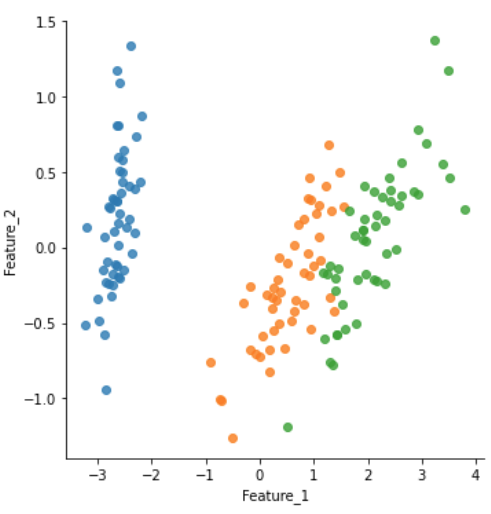
\includegraphics[width=8.0cm]{./pic/Clustering_Beispiel.png}
    \caption{Beispiel für Clustering}
    \label{fig:Clustering_Beispiel}
\end{figure}

Bei der ,,\textit{Dimensionality Reduction}'' versucht der Algorithmus das Datenset in einer 
Dimensionalität, also seiner Anzahl an Feldern, zu reduzieren. Es wird also die Frage gestellt, 
ob das bestehende Datenset auch mit weniger Feldern Abhängigkeiten feststellen lässt. Dieser 
Schritt wird vorallem für Modelle benutzt, die sensibel gegenüber hoher Dimensionalitäten sind, 
sodass das Datenset vor dem Training in seiner Dimensionalität heruntergebrochen werden kann.

Im Rahmen des Projektes wurden hauptsächlich Klassifizierungs-Algorithmen genutzt, da ein Großteil der 
Datensets Labels zur Überprüfung hatte. Um einen Vergleich herzustellen werden später trotzdem noch 
einzelne Ergebnisse von Clustering und Dimensionality Reduction betrachtet. Im folgenden sollen die genutzten 
Modelle erklärt werden.

\subsection{Random Forest Classifier}

Random Forests stellen eine Unterkategorien der ,,\textit{Decision Trees}'' dar. Decision Trees sind einfache
Anordnungen von bestimmten Fragen, die über das Datenset gestellt werden, um eine Klassifikation zu erreichen.

\begin{figure}[h]
    \centering
    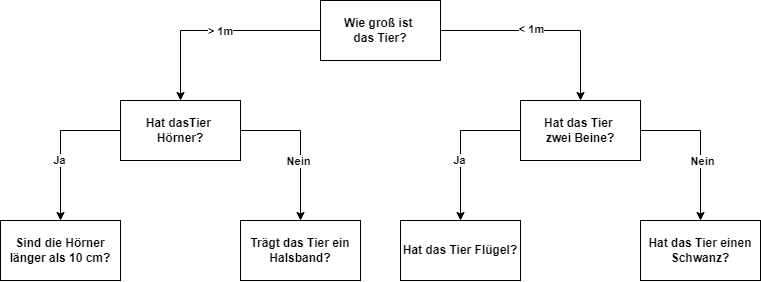
\includegraphics[width=10.0cm]{pic/DecisionTree.png}
    \caption{Beispiel eines Decision Trees}
    \label{fig:DT_Beispiel}
\end{figure}

Erstellt man ein ,,\textit{Ensemble}'' aus Decision Trees die Erwartungen über einen zufällig gewählten 
Teil des Datensets treffen können, entsteht ein Random Forest.
Der Random Forest Classifier versucht, eine Menge einfacher Schätzfunktionen über einen komplexeren 
Sachverhalt ,,abstimmen'' zu lassen. Während sich in einem einzelnen Entscheidungsbaum Fehleinschätzungen 
entwickeln können, sinkt die Chance auf eine solche Fehleinschätzung, je mehr unabhängige 
Entscheidungsbäume man befragt. 

\subsection{Support Vector Classifier}
Der Support Vector Classifier(SVC) versucht in einem Datenset anhand von bestimmten Cut-Off-Values klare Grenzen 
zwischen Werten zu finden, sodass man alle Messwerte ober- und unterhalb der Grenze eindeutig Klassifizieren 
kann.

\begin{figure}[h]
    \centering
    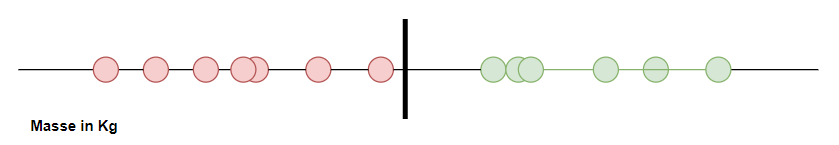
\includegraphics[width=10.0cm]{pic/SVC_1D.png}
    \caption{Beispiel eines Support Vector Classifiers}
    \label{fig:SVC_1D}
\end{figure}

In Abb. \ref{fig:SVC_1D} ist der SVC ein Punkt auf einer eindimensionalen Linie, auf der das Gewicht in Kg von z.B. 
Mäusen in ,,Unter-'' und ,,Übergewichtig'' unterteilt wird. Dieser Punkt ist Ergebnis aller Verhältnisse der einzelnen
Datenpunkte zueinander. Durch sog. ,,\textit{Kernel Funktionen}'' versucht der Algorithmus nun Beziehungen 
in höheren Dimensionen zu finden, wie z.B. $Masse^2$, $Masse^3$ usw. .\\
Da der SVC die Verhältnisse aller Datenpunkte zueinander betrachtet, ist er sehr anfällig für Ausreißer in 
den Daten, was während der Projektarbeit, auch bezüglich anderer Klassifizierungsmethoden, berücksichtigt wurde.

\subsection{Gradient Boosting Classifier}


\subsection{Bagging Classifier}

\subsection{Neural Networks}

\subsection{Long Short Term Memory}

\section{CO2 als Anwesenheitsindikator}\label{CO2}

Der CO2-Gehalt der Raumluft ist als sehr guter Indikator für menschliche Präsenz anzusehen. Anders als andere 
Umweltindikatoren wie Temperatur oder Luftfeuchtigkeit hat der CO2-Gehalt die Eigenschaft, dass es in 
geschlossenen Räumen keine äußeren Einflussfaktoren für diesen Messwert gibt. In einem Büroraum kann der 
Mensch als alleinige Quelle für CO2 angesehen werden.\\
Der Anteil an CO2 in der Atemluft beträgt zwischen 350 und 450 ppm. Es gibt in Deutschland und auch Europa 
keine grundsätzlich festgelegten Grenzwerte für akzeptable Raumluft, vielmehr raten Gesundheitsämter 
verschiedener Länder Grenzwerte zwischen 1200 und 1500 ppm einzuhalten. Bei der Obergrenze von 1500 ppm 
entstehen beim Menschen erste Müdigkeitserscheinungen, weshalb dieser Wert in der Literatur als maximaler 
Richtwert für Innenräume gilt. 

\section{Outlier Detection}

\begin{align}
(p_i * p_j)(n) & =  \sum_{k \in \mathbb{D}} p_i(k) \cdot p_j(n - k) \\
p_{total} & =  p_0 \ast p_1 \ast \ldots p_{n-1}; \forall n
\end{align}

% Formel
Hier ist nur eine einfache Formel mit der \texttt{equation}-Umgebung für die Minkowski Metrik:
\begin{equation}\label{Minkowski}
D\left(X,Y\right)=\left(\sum_{i=1}^n |x_i-y_i|^p\right)^{1/p}\\
\end{equation}

Wie in Gleichung \ref{Minkowski} zu erkennen ist, ergibt sich die L2-Norm (Euklidische Distanz), wenn man den Exponenten $p = 2$ wählt.

Support Vector Machines \cite{Haykin99} nutzen die Euklidische Distanz (oder äquivalent) das Skalarprodukt.
%% Zwei Abbildungen, die zusammen gehören

%\begin{figure}
%        \centering
%        \begin{minipage}[c]{0.45\textwidth}
%                \includegraphics[height=6.5cm]{pic/dateiname1.png}
%        \end{minipage}
%        \begin{minipage}[c]{0.45\textwidth}
%                \includegraphics[height=6.5cm]{pic/dateiname2.png}
%        \end{minipage}
%        \caption{Zwei Abbildungen}\label{fig:zwei_abb}
%\end{figure}
